\section{Estructura de la Base de Datos}
La base de datos TRANSACCIONALIDAD contiene una tabla principal llamada MOVIMIENTOS con la siguiente estructura:
\begin{comando}	{Creación de tabla MOVIMIENTOS}
	\begin{verbatim}
		CREATE TABLE MOVIMIENTOS(
			IDMOVIMIENTOS INTEGER NOT NULL IDENTITY (1,1),
			MONTO MONEY NOT NULL,
			DEPOSITO_RETIRO CHAR(1) NOT NULL,
			PRIMARY KEY (IDMOVIMIENTOS)
		);
	\end{verbatim}	
\end{comando}
Los datos fueron generados mediante el siguiente procedimiento almacenado:
\begin{comando}	{Creación de PROCEDURE}
	\begin{verbatim}
			CREATE PROCEDURE INSERTA_MOVIMIENTOS
			AS
			DECLARE @DATO INTEGER;
			DECLARE @CONTADOR INTEGER;
			BEGIN TRANSACTION
				SET @CONTADOR=1;
				WHILE @CONTADOR <= 10000000
				BEGIN
				SET @DATO = ROUND(RAND() * 999999, 0);
				INSERT INTO MOVIMIENTOS
				(MONTO, DEPOSITO_RETIRO)
				VALUES (@DATO, 'D');
				SET @CONTADOR = @CONTADOR + 1;
			END;
			IF @@ERROR <> 0
				ROLLBACK TRANSACTION;
			ELSE
			COMMIT TRANSACTION;
	\end{verbatim}	
\end{comando}
\section{Análisis Estadístico}
A continuación se presentan los diversos cálculos estadísticos realizados sobre los datos de la tabla MOVIMIENTOS.
\subsection{Promedio (Media Aritmética)}
El promedio representa la suma de todos los valores dividida por el número de observaciones. La consulta SQL utilizada es:
\begin{comando} {Calculado el Promedio:}
	\begin{verbatim}
		SELECT AVG(MONTO) AS Promedio FROM MOVIMIENTOS;
	\end{verbatim}
\end{comando}
Matemáticamente, el promedio se define como:
\begin{equation}
	\bar{x} = \frac{1}{n}\sum_{i=1}^{n}x_i
\end{equation}
Donde:
\begin{itemize}
	\item $\bar{x}$ es la media aritmética
	\item $n$ es el número total de observaciones
	\item $x_i$ es el valor de la i-ésima observación
\end{itemize}
\subsection{Moda}
La moda es el valor que aparece con mayor frecuencia en un conjunto de datos. La consulta SQL para obtener la moda es:
\begin{comando} {Calculando la Moda:}
	\begin{verbatim}
		SELECT TOP 1 MONTO AS Moda,
			COUNT(MONTO) AS Frecuencia 
			FROM MOVIMIENTOS 
			GROUP BY MONTO ORDER BY
		Frecuencia DESC;
	\end{verbatim}
\end{comando}
Esta consulta:
\begin{enumerate}
	\item Agrupa los datos por el valor de MONTO
	\item Cuenta la frecuencia de cada valor
	\item Ordena de mayor a menor frecuencia
	\item Selecciona el primer valor, que corresponde al más frecuente
\end{enumerate}
\subsection{Valor Mínimo}
El valor mínimo es el menor valor presente en el conjunto de datos:
\begin{comando}{Calculando el Mínimo:}
	\begin{verbatim}
		SELECT MIN(MONTO) AS Minimo FROM MOVIMIENTOS;
	\end{verbatim}
\end{comando}
\subsection{Valor Máximo}
El valor máximo es el mayor valor presente en el conjunto de datos:
\begin{comando}{Calculando el Máximo:}
	\begin{verbatim}
		SELECT MAX(MONTO) AS Maximo FROM MOVIMIENTOS;
	\end{verbatim}
\end{comando}
\subsection{Mediana}
La mediana es el valor que divide el conjunto de datos ordenados en dos partes iguales. Para calcular la mediana en SQL Server, se utilizó la siguiente consulta:
\begin{comando}{Calculando la Mediana:}
	\begin{verbatim}
		WITH OrderedData AS (
			SELECT MONTO,
				ROW_NUMBER() OVER (ORDER BY MONTO) AS RowAsc,
				ROW_NUMBER() OVER (ORDER BY MONTO DESC) AS RowDesc
			FROM MOVIMIENTOS
		)
		SELECT
			AVG(MONTO) AS Mediana
		FROM OrderedData WHERE 
			RowAsc = RowDesc OR 
			RowAsc + 1 = RowDesc OR 
			RowAsc = RowDesc + 1;
	\end{verbatim}
\end{comando}
Esta consulta:
\begin{enumerate}
	\item Crea una tabla temporal (CTE) con los datos ordenados
	\item Asigna números de fila tanto en orden ascendente como descendente
	\item Selecciona los valores centrales donde las filas ascendentes y descendentes se encuentran
	\item Calcula el promedio (por si hay un número par de elementos)
\end{enumerate}
Para un conjunto de datos con $n$ elementos:
\begin{itemize}
	\item Si $n$ es impar, la mediana es el elemento en posición $\frac{n+1}{2}$
	\item Si $n$ es par, la mediana es el promedio de los elementos en posiciones $\frac{n}{2}$ y $\frac{n}{2}+1$
\end{itemize}
\section{Análisis de Tendencia}
Para analizar la tendencia de los datos, se realizaron dos pasos:
\subsection{Representación en Coordenadas (x,y)}
Primero, se obtuvieron pares ordenados donde $x$ es el ID del movimiento y $y$ es el monto:
\begin{comando}{Obteniendo Coordenadas (x,y):}
	\begin{verbatim}
		SELECT
			IDMOVIMIENTOS AS X,
			MONTO AS Y
		FROM MOVIMIENTOS;
	\end{verbatim}
\end{comando}
\subsection{Cálculo de la Pendiente}
Para determinar la tendencia, se calculó la pendiente de la recta de regresión lineal:
\begin{comando}{Calculando la Pendiente:}
	\begin{verbatim}
		WITH Data AS (
			SELECT
				IDMOVIMIENTOS AS X,
				MONTO AS Y
			FROM MOVIMIENTOS
		)
		SELECT
			(COUNT() * SUM(X * Y) - (SUM(X) * SUM(Y))) / 
			(COUNT() * SUM(X * X) - SUM(X) * SUM(X)) 
			AS Pendiente
		FROM Data;
	\end{verbatim}
\end{comando}
La pendiente se calcula utilizando el método de mínimos cuadrados, cuya fórmula es:
\begin{equation}
	m = \frac{n\sum_{i=1}^{n}x_i y_i - \sum_{i=1}^{n}x_i \sum_{i=1}^{n}y_i}{n\sum_{i=1}^{n}x_i^2 - (\sum_{i=1}^{n}x_i)^2}
\end{equation}
Donde:
\begin{itemize}
	\item $m$ es la pendiente de la recta de regresión
	\item $n$ es el número de pares $(x,y)$
	\item $x_i$ y $y_i$ son los valores del i-ésimo par
\end{itemize}
La interpretación de la pendiente es la siguiente:
\begin{itemize}
	\item Si $m > 0$, hay una tendencia creciente
	\item Si $m < 0$, hay una tendencia decreciente
	\item Si $m \approx 0$, no hay una tendencia clara
\end{itemize}
\section{Interpretación de Resultados}
Los resultados obtenidos de los cálculos anteriores proporcionan información valiosa sobre la distribución y comportamiento de los montos en la tabla MOVIMIENTOS:
\begin{itemize}
	\item El \textbf{promedio} indica el valor central desde una perspectiva aritmética.
	\item La \textbf{moda} muestra el valor más común, lo que puede indicar montos de transacción frecuentes.
	\item Los valores \textbf{mínimo} y \textbf{máximo} definen el rango completo de los datos.
	\item La \textbf{mediana} proporciona un valor central robusto, menos afectado por valores extremos que el promedio.
	\item La \textbf{pendiente} de la recta de regresión indica si existe alguna tendencia temporal en los montos a medida que se registran nuevos movimientos.
\end{itemize}
Dado que los datos fueron generados aleatoriamente con valores entre 0 y 999,999, se esperaría:
\begin{itemize}
	\item Un promedio cercano a 500,000
	\item Una distribución relativamente uniforme sin una moda pronunciada
	\item Una mediana también cercana a 500,000
	\item Una pendiente cercana a cero, indicando ausencia de tendencia
\end{itemize}

\section{Representación grafica mediante Power Bi}

Utilizando la herramienta Power BI se creo una representación de los datos donde el eje X corresponde a ID del MOVIMIENTO y el eje Y corresponde a el MONTO del deposito.

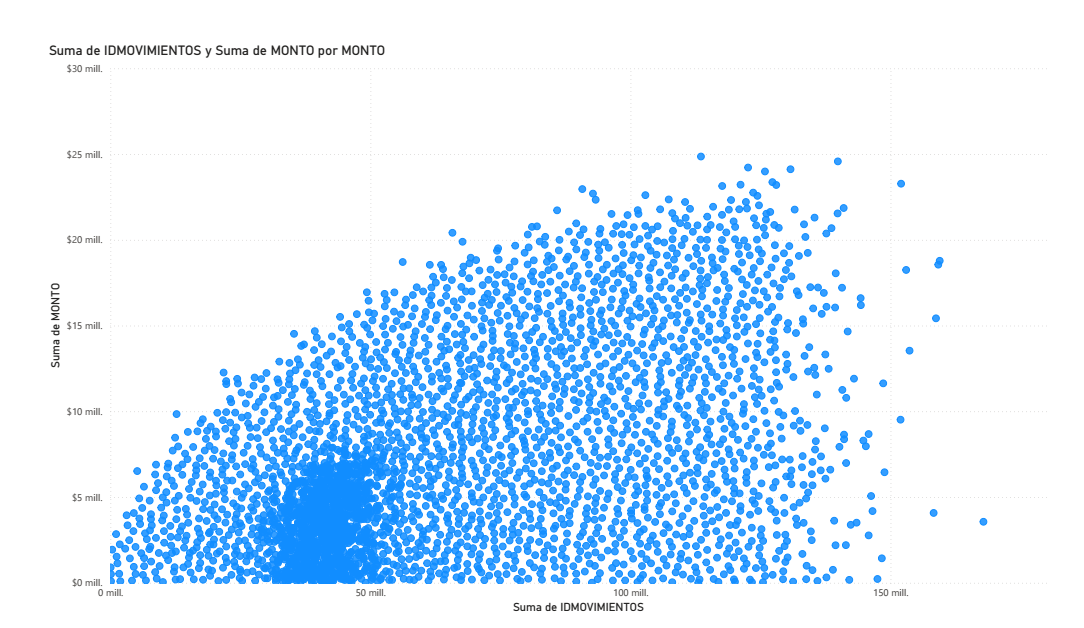
\includegraphics[width=\textwidth, keepaspectratio]{imagenes/powerbi}

\section{Extracción, Transformación y Carga de Datos (ETL)}

\subsubsection{Pandas}
Pandas es una de las bibliotecas más utilizadas en Python para la manipulación y análisis de datos. Proporciona estructuras de datos flexibles como DataFrame y Series, facilitando la limpieza, transformación y preparación de datos \cite{mckinney2010pandas}.

\begin{itemize}
	\item Manipulación de datos tabulares.
	\item Soporte para archivos CSV, Excel, JSON y bases de datos SQL.
	\item Métodos eficientes para filtrado, agregación y procesamiento de datos.
\end{itemize}

\subsubsection{NumPy}
NumPy proporciona soporte para arrays multidimensionales y funciones matemáticas avanzadas. Es fundamental para cálculos numéricos eficientes \cite{harris2020array}.

\begin{itemize}
	\item Soporte para operaciones matriciales.
	\item Funciones matemáticas optimizadas.
	\item Base para otras bibliotecas como Pandas y Scipy.
\end{itemize}

\subsubsection{PySpark}
PySpark es una interfaz de Apache Spark para Python, diseñada para procesar grandes volúmenes de datos en entornos distribuidos \cite{zaharia2016apachespark}.

\begin{itemize}
	\item Procesamiento de datos en paralelo.
	\item Manejo de datos en clústeres.
	\item Integración con otras herramientas de Big Data.
\end{itemize}

\subsubsection{SQLAlchemy}
SQLAlchemy es un ORM (Object-Relational Mapping) que permite interactuar con bases de datos SQL de manera eficiente \cite{bayer2010sqlalchemy}.

\begin{itemize}
	\item Abstracción de consultas SQL en Python.
	\item Conexión a múltiples bases de datos.
	\item Optimización de consultas y transacciones.
\end{itemize}

\subsubsection{Requests}
Requests es una biblioteca en Python utilizada para hacer solicitudes HTTP de manera sencilla y eficiente \cite{reitz2011requests}.

\begin{itemize}
	\item Extracción de datos desde APIs REST.
	\item Manejo de autenticación y sesiones.
	\item Soporte para solicitudes GET, POST, PUT y DELETE.
\end{itemize}

\subsubsection{BeautifulSoup y Scrapy}
BeautifulSoup y Scrapy son herramientas populares para la extracción de datos desde páginas web \cite{richardson2007beautifulsoup}.

\begin{itemize}
	\item Scrapy permite la automatización del web scraping.
	\item BeautifulSoup facilita la manipulación del HTML y XML.
	\item Soporte para navegación y extracción estructurada de datos.
\end{itemize}

\subsection{Visualización de Datos}

\subsubsection{Matplotlib}
Matplotlib es una biblioteca para la creación de visualizaciones estáticas en Python. Proporciona una interfaz similar a MATLAB para generar gráficos \cite{hunter2007matplotlib}.

\begin{itemize}
	\item Creación de gráficos de líneas, barras y dispersión.
	\item Personalización de ejes, colores y etiquetas.
	\item Exportación en formatos PNG, SVG y PDF.
\end{itemize}

\subsubsection{Seaborn}
Seaborn está basado en Matplotlib y permite la creación de gráficos estadísticos con mejor diseño y mayor facilidad \cite{waskom2021seaborn}.

\begin{itemize}
	\item Visualizaciones avanzadas de datos categóricos y numéricos.
	\item Integración con Pandas para análisis rápido.
	\item Gráficos de correlación y distribución de datos.
\end{itemize}

\subsubsection{Plotly}
Plotly es una biblioteca para la generación de visualizaciones interactivas, adecuada para dashboards y aplicaciones web \cite{plotly2021}.

\begin{itemize}
	\item Creación de gráficos 3D y animaciones.
	\item Integración con Dash para dashboards interactivos.
	\item Soporte para mapas geoespaciales y diagramas avanzados.
\end{itemize}

\subsubsection{Bokeh}
Bokeh permite la generación de gráficos interactivos con alto rendimiento \cite{bokeh2018}.

\begin{itemize}
	\item Creación de dashboards en navegadores web.
	\item Visualización de grandes volúmenes de datos.
	\item Personalización avanzada de gráficos.
\end{itemize}

\subsubsection{Dash}
Dash es un framework basado en Flask que permite la creación de dashboards interactivos \cite{plotly2017dash}.

\begin{itemize}
	\item Construcción de aplicaciones web con visualizaciones.
	\item Integración con Plotly para interactividad.
	\item Ideal para compartir análisis de datos.
\end{itemize}

